\section{METODOLOGÍA}

Como lo demuestra el "No Free Luch Theorem" no existe un mejor algoritmo para cada categoría de problemas en Machine Learning.  Por eso es que vamos a estudiar varios y decidir cuál, o la combinación de cuáles nos brinda un mejor modelo para predecir un nuevo evento siguiendo el set de datos de la competencia.
Comenzaremos con algoritmos simples y de a poco intentremos refinarlos.

\subsection{Limpieza y Preparación de los Datos}
Antes de comenzar la construcción de cualquier modelo es fundamental realizar esta etapa. La preparación de los datos es difícil, debemos definir cuál es la mejor forma de manejarlos para describir el problema.

Wickham señala que no es un proceso de una sola vez, que es iterativo como entender el problema más profundo en cada paso sucesivo. El objetivo es estructurar los datos para facilitar el análisis de datos.\cite{RforDataScience}




Dado a que para el algoritmo solo vamos a manejar variables numéricas
\begin{itemize}
   \item Eliminamos la columna de start\_station\_name y dejamos start\_station\_id.
    
    \item Eliminamos la columna de end\_station\_name y dejamos start\_station\_id.
    
    \item En subscription\_type tenemos dos posibles valores, 
    subcriber o customer el primero será 1 y el segundo 2.
    
    \item
    
\end{itemize}

Utilizaremos una técnica simple en la que sustituimos cada valor faltante por la mediana de todos los valores presentes.


\subsection{Sckit-Learn}

En nuestra búsqueda de información y recomendaciones para el desarrollo de nuestro modelo encontramos Sckit learn, una librería para Python. 
En la documentación figura una diagrama que nos guía para encontrar posibles estimadores para nuestro problema.

\begin{figure}[h]
\centering
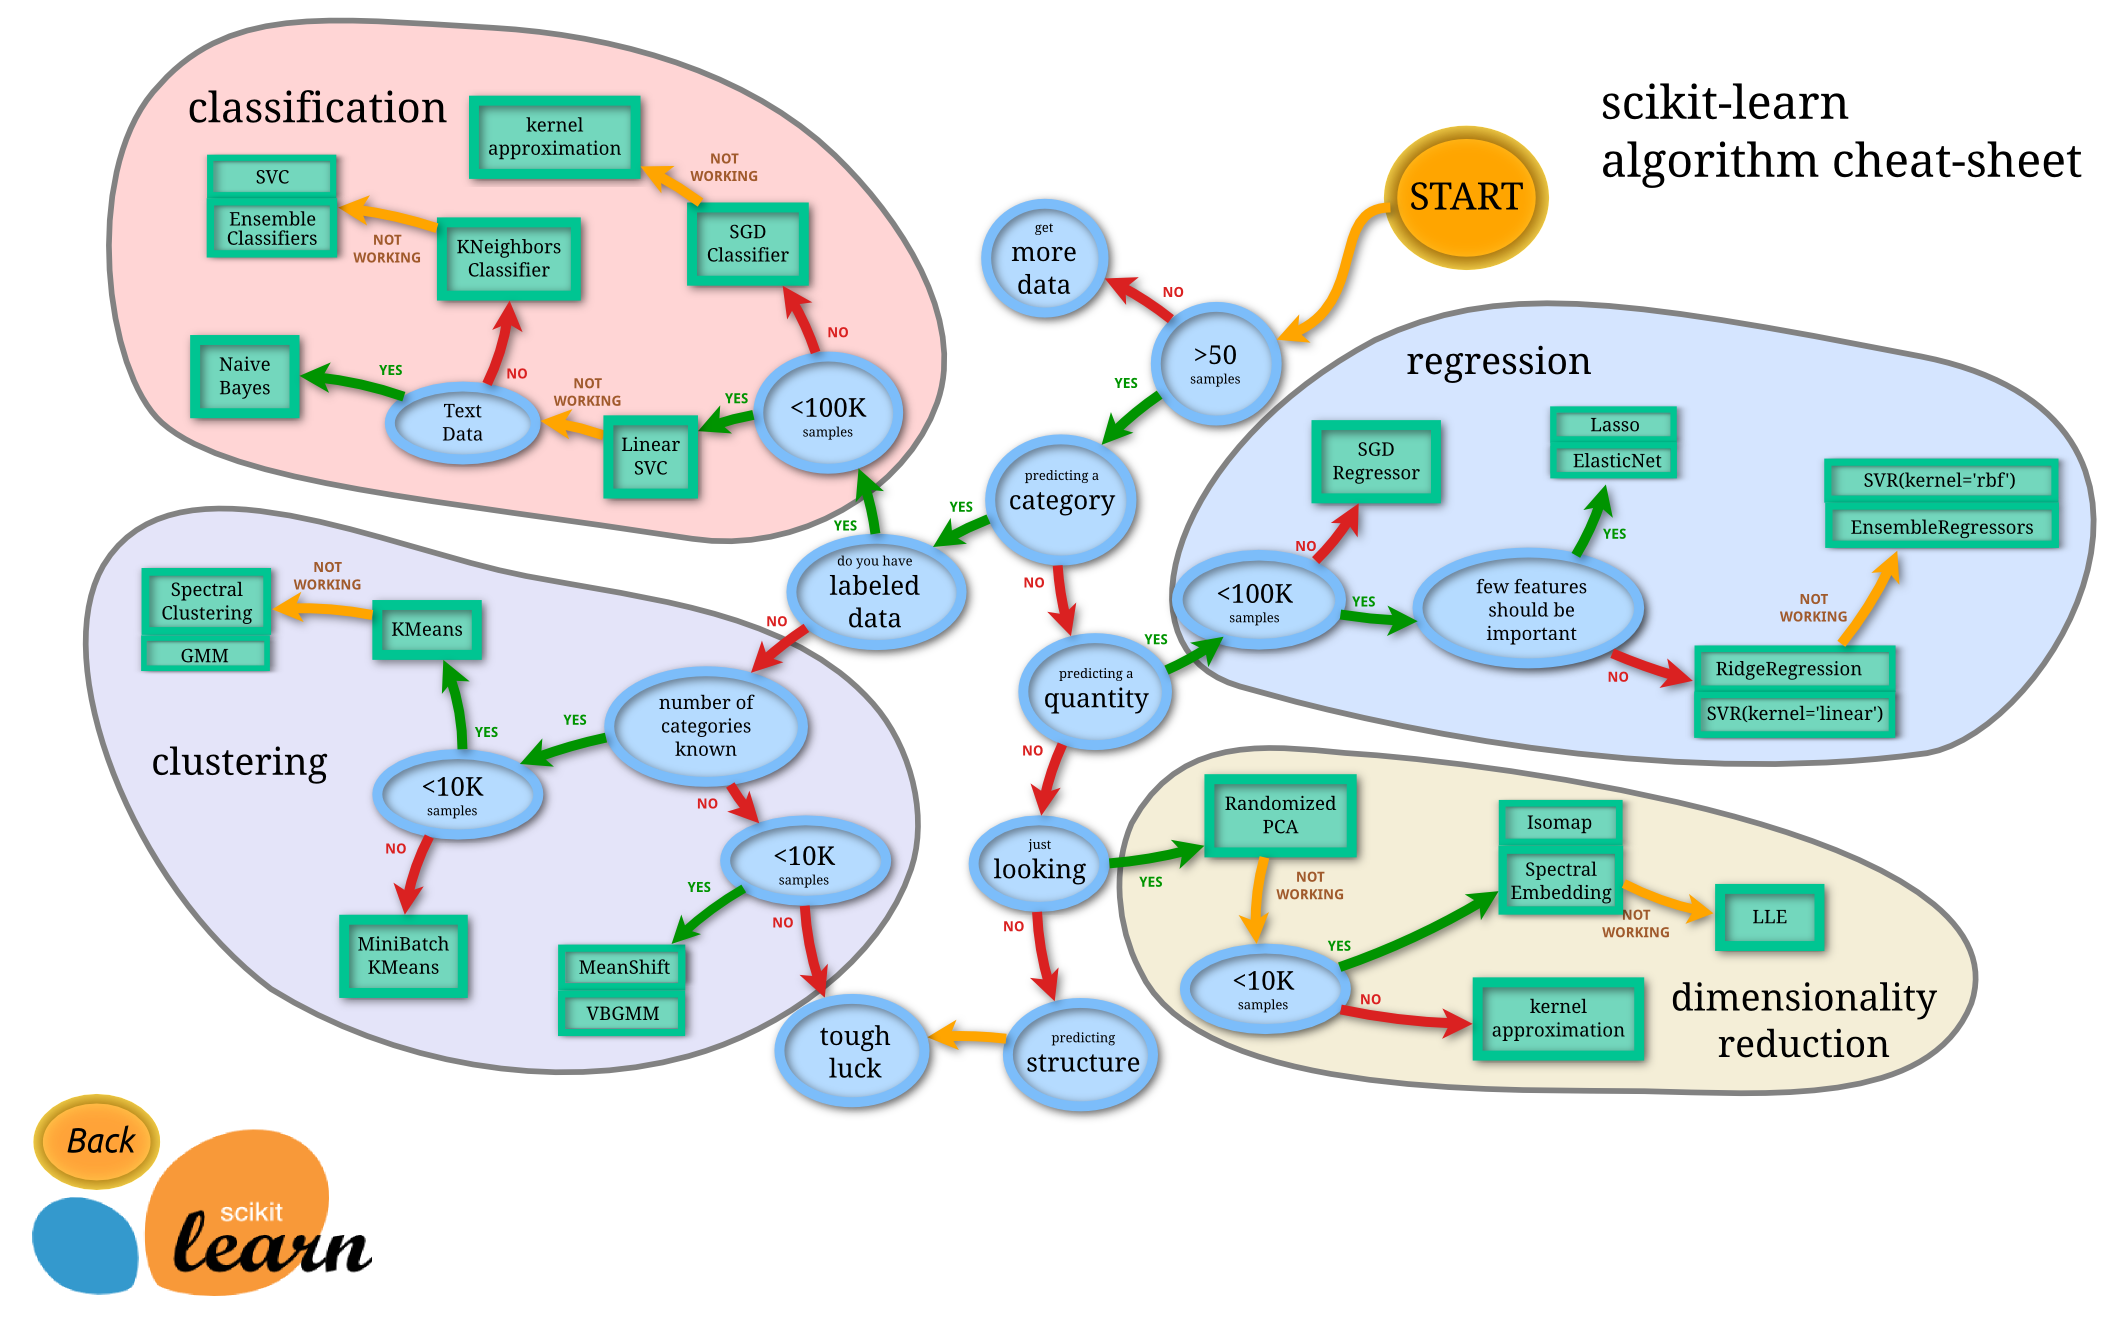
\includegraphics[height=10cm]{imagenes/sckit.png}
\label{fig:exemplo}
\end{figure}

\subsection{SGD Regresor}
Dado a que tenemos una cantidad de datos mucho mayor a 100k probaremos con SGD Regresor


\begin{table}[h]
\centering
\caption{ Modelo de como as tabelas devem ser inseridas no texto }
\vspace{0.2in}
\newcolumntype{C}{>{\centering\arraybackslash}X}%
\newcommand{\rowstyle}[1]{%
  \protected\gdef\currentrowstyle{#1}%
}
\begin{tabularx}{\textwidth}{>{\bf}C|C|C|C}
\hline 
\textbf {Índice} & \textbf{Coluna 01} &\textbf{ Coluna 02} & \textbf{Coluna 03} \\ \hline \hline
Linha 01 & & & \\ \hline
Linha 02 & & & \\ \hline                         

\end{tabularx}
\end{table}






\begin{table}[h]
\centering
\caption{ Modelo de como as tabelas devem ser inseridas no texto }
\vspace{0.2in}
\newcolumntype{C}{>{\centering\arraybackslash}X}%
\newcommand{\rowstyle}[1]{%
  \protected\gdef\currentrowstyle{#1}%
}
\begin{tabularx}{\textwidth}{>{\bf}C|C|C|C}
\hline 
\textbf {Índice} & \textbf{Coluna 01} &\textbf{ Coluna 02} & \textbf{Coluna 03} \\ \hline \hline
Linha 01 & & & \\ \hline
Linha 02 & & & \\ \hline                         

\end{tabularx}
\end{table}